\documentclass[letterpaper,12pt]{article}
\usepackage[letterpaper, margin=2.54cm]{geometry}
%\usepackage{harvard}


%\usepackage[round,sort,authoryear]{natbib}
%\bibliographystyle{plainnat} 
%\setlength{\bibsep}{0pt plus 0.3ex}
%\bibliographystyle{agsm}
%\bibliographystyle{plainnat}      % or abbrvnat/unsrtnat, etc.

\usepackage[natbib=true, style=authoryear, backend=bibtex8, useprefix=true, maxbibnames=99, mincitenames=1, maxcitenames=2, labeldate=year]{biblatex} 

\addbibresource{bibs/survey-methodology.bib}


\usepackage{enumitem}
\usepackage{arydshln}
%\usepackage[backend=biber, citestyle=authoryear, bibencoding=utf8]{biblatex}
%\addbibresource{./bibs/adaptive-sampling.bib}
%\addbibresource{./bibs/survey-methodology.bib}
\usepackage{todonotes}
\usepackage{comment}

\usepackage{amsmath, amsthm, amsfonts, mathtools, csquotes, bm, centernot, bbm, multirow, rotating, lscape}
\usepackage[toc,page]{appendix}
\usepackage{booktabs}
\usepackage[T1]{fontenc}


\usepackage{hyperref}
\hypersetup{
    colorlinks=true,
    citecolor=blue,
    linkcolor=blue,
    filecolor=magenta,      
    urlcolor=blue,
    pdftitle={Overleaf Example},
    pdfpagemode=FullScreen,
    }
    

\usepackage[onehalfspacing]{setspace}

\usepackage{algorithm}
\usepackage{algpseudocode}
\theoremstyle{proposition}
\newtheorem{proposition}{Proposition}[section]
\newtheorem{prop}{Proposition}

\usepackage{pgf, tikz}
\usetikzlibrary{arrows, automata}

\usepackage[onehalfspacing]{setspace}



\DeclareMathOperator*{\argmax}{argmax}
\DeclareMathOperator*{\argmin}{argmin}
%\title{Continuous Survey Sample Optimization \\ Using Ad Platform APIs}
%\title{Leveraging Digital Ad Platforms for Survey Sampling}
%\title{Leveraging Ad Platforms to Optimize Survey Sampling}
%\title{Online Survey Recruitment with \\  Ad Platform Optimization}
%\title{Optimizing Survey Recruitment with Ad Platforms}
%\title{Continuous Survey Sample Optimization \\ Using Ad Platforms}
%\title{Leveraging Ad Platforms for \\ Continuous Survey Sample Optimization}
%\title{Dynamic Survey Sample Optimization \\ Using Advertising Platforms}
%\title{{Adaptive Survey Recruitment \\ via Advertising Platforms}
\title{{\Huge Adaptive Survey Sampling  via Ad Platforms}\thanks{The authors thank participants at the MIT Conference on Digital Experimentation (CODE), the Workshop on Frontiers in Measurement and Survey Methods, the Marketing Science Conference, the China India Insights Program, the AIML and Business Analytics Conference, and the MarkTech Conference for their valuable feedback. Dante Donati declares no competing interests. Nandan Rao  has ownership interests in Virtual Lab LLC, a company that applies the open-source methodology described in this paper to provide paid services. This research received ethical clearance from the Columbia University IRB (AAAV1539). All data and code underlying our analyses can be made available to ensure transparency and replicability. All remaining errors are the authors’ own.\vspace{1pt}}}


\begin{document}

\author{\vspace*{1cm}{\Large Dante Donati}\thanks{Columbia Business School and CESifo, dd3137@gsb.columbia.edu} \hspace{50pt} {\Large  Nandan Rao}\thanks{Virtual Lab and Universitat Autònoma de Barcelona, nandan@vlab.digital}}

\date{September 15, 2025}
\maketitle
\singlespacing
\begin{abstract}
This paper introduces and validates a new methodology for recruiting highly stratified survey respondents using digital advertising platforms. Our approach leverages ad platform APIs with a novel algorithm that dynamically optimizes participant recruitment in real time by minimizing the variance of post-stratification weighted estimates. We demonstrate the method’s efficacy through a 1,500-person U.S. study, benchmarking results against gold-standard surveys (GSS, CPS, Pew), a leading online panel provider (Prolific), and an LLM-based synthetic methodology (digital twins). We obtain a mean absolute deviations of 6.1 percentage points from the gold-standard benchmarks, improving on both the online panel provider and LLM-based approaches. We show that this methodology is both cost-effective in the U.S., with a total cost of \$0.30 per question per respondent, but also deployable around the world in both developed and emerging economies, where we provide evidence of success in over 33 studies across 23 countries. We present the software as an open-source platform, deployable as a web application on both public and private clouds.



%Our methodology provides a novel and convenient way to gather consumer insights, enabling the collection of highly targeted, cost-effective samples in both developed economies and emerging markets.



%\noindent JEL Codes: I12, I31, L82, L86\\
%\vspace{-20pt}
\vspace{0.3cm}
%\noindent Keywords: Ad Platforms, Consumer Insights,  Online Sampling, Survey Research
\noindent \textit{Keywords: Ad Platforms, APIs, Consumer Insights,  Online Sampling, Survey Research}

%By reaching billions of people everyday, digital Ad platforms such as Google, Facebook and Instagram offer researchers and practitioners unprecedented opportunities to recruit survey respondents and conduct studies entirely online. Researchers have successfully gathered “convenience samples” by creating ads for targetable populations. However, by manually creating these ads, researchers are limited to the explicit targeting criteria available on the platform as well as limited in the complexity of stratification which is feasible. We formulate the problem of dynamically setting ad budgets for survey sample collection as one of minimizing the variance of a post-stratification weighted expectation subject to budget constraints. We use this technique to replicate some questions from well-established social science surveys in the US, including the General Social Survey (GSS) and the Current Population Survey (CPS). We analyze the differences between our survey responses and those of the major social surveys and validate the accuracy and efficiency of our technique, with mean absolute deviations ranging around 6.3 p.p., and a cost per question per respondent around \$0.30. Finally, we present the software as an open-source platform that can be deployed as a web application on public or private clouds. Our methodology offers a novel and convenient approach to gather consumer insights, enabling the collection of highly targeted, cost-effective samples in developed economies and emerging markets.

%LONGER VERSION
%By reaching billions of people everyday, digital advertising platforms such as Google and Meta offer researchers and advertisers unprecedented opportunities to gather survey responses and conduct studies entirely online. Researchers have successfully recruited “convenience samples” by creating ads for targetable populations. However, by manually creating these ads, researchers are limited to the explicit targeting criteria available on the platform as well as limited in the complexity of stratification which is feasible. We formulate the problem of dynamically setting ad budgets for survey sample collection as one of minimizing the variance of a post-stratification weighted expectation subject to budget constraints. We then show that this problem can be continuously optimized, in real-time, by building software that connects to both the APIs of the ad platforms and to the API of a survey platform. We use this technique to replicate some questions from major social science surveys in the US and India, including the General Social Survey (GSS), the Current Population Survey (CPS) and the National Family Health Survey (NFHS). We analyze the differences between our survey responses and those of the major surveys to validate the potential accuracy of our technique. Overall, our results indicate that this methodology has broad applications for researchers and organizations interested in studying socioeconomic outcomes and consumer behavior, including the collection of both nationally representative and highly-targeted samples. The flexibility and scalability of this method make it particularly suitable for time-sensitive studies, where traditional methods might be too slow or expensive. Additionally, we present the software as an open-source platform that can be deployed as a web application on public or private clouds.
\end{abstract}

\clearpage
\onehalfspacing

\begin{comment}
\section{Notes}

1. Results from the American surveys. 
    a. Compare demographics. 
    b. Compare our MAD in all questions. 
    c. Discuss differences. 
    d. Uses post-stratification weighting 
        i. https://www.cambridge.org/core/journals/political-analysis/article/abs/bayesian-multilevel-estimation-with-poststratification-statelevel-estimates-from-national-polls/22A5EF78D027E76C782B3280D400FCC9
        ii. https://academic.oup.com/jssam/article-abstract/8/1/4/5699631

    e. Comparison with naive recruitment

2. Expand work in other countries: scope of the grant. INTO GRANT
    a. India (DHS)
    b. Other countries with good/recent DHS data.
    c. One other country with no DHS data.

3. Improvements in stratification:
    a. Automatic exclusions (turn on and off based on the optimization): right now the optimizer it is not incorporating that. INTO GRANT
    b. Optimize for survey completions (right now is CTR on survey). INTO GRANT
    
    c. Learning stratifying variables: NOT IN GRANT, BUT MENTION IT
        i. Bayesian post-stratification model in the optimization: bringing in the analysis
        ii. Dynamically learning which variables matter: https://arxiv.org/abs/2204.05793, (extension of this algorithm: https://proceedings.mlr.press/v89/atan19a.html)

4. Improvements in survey platform (Fly): NOT IN GRANT
    i. Whatsapp
    ii. Payments in certain countries
    iii. Conversational surveys (GenAI)

More info here: https://docs.google.com/document/d/1BfTV7hpzKHBkpnkaej5xidRdYOa8yLBdSv5EJydv4zQ/edit?tab=t.0

\end{comment}

\section{Introduction}
Surveys play a fundamental role in understanding human behavior, consumer preferences, and societal trends, making them indispensable tools across various domains in academia, industry, and public policy.\footnote{Surveys are widely used in social science research, including Political Science, Economics, Sociology, Marketing, and Management. Industry practitioners rely on survey research to inform product design, demand forecasting, branding effectiveness, and other key decisions, while institutions use them to understand citizens' needs and emerging trends (\citealt{rossi2013handbook, vannette2017palgrave}).} In the mid-20th century, the widespread adoption of telephones and the advent of random digit dialing (RDD) revolutionized data collection by enabling researchers to reach large and diverse populations while addressing sampling biases (\citealt{Cooper1964,Glasser1972,sudman1973uses}). However, in the 21st century, declining response rates made traditional RDD methods increasingly inadequate and expensive (\citealt{keeter2017low}). By contrast, the emergence of internet-based platforms provides researchers and practitioners with innovative ways to connect with target audiences (\citealt{yeager2011comparing}). 


Online panels offered by platforms like Prolific and Amazon Mechanical Turk (MTurk) have become increasingly popular for survey recruitment due to their cost-effectiveness and ability to quickly assemble participant samples. However, their utility is constrained by two critical limitations. First, they are geographically bounded, with respondent pools concentrated in the United States and a few other developed countries, leaving researchers unable to gather insights from crucial emerging markets \citep{narasimhan2015marketing}.\footnote{Relatedly, these panels often produce samples that are disproportionately composed of certain demographic groups, such as younger, more educated, and tech-savvy individuals, leading to challenges in achieving broad population coverage \citep{stewart2015average}.} Second, because these respondent pools are pre-determined, they present challenges in achieving coverage for specific populations that may be of interest to researchers (\citealt{peer2017beyond}).\footnote{This can have significant implications for research outcomes, as failing to account for omitted moderators, including demographic and contextual differences, may lead to unexplained variability in effect sizes across studies (\citealt{krefeld2024exposing}).}

Researchers have increasingly turned to social media  such as Facebook and Instagram to recruit participants for surveys. Advertising platforms of social media enable a broad reach while allowing for precise demographic targeting. However, unlike pre-assembled panels, recruitment through digital ads requires researchers to actively design and monitor campaigns, optimize ad placement, and manage budget allocations to achieve desired sampling outcomes (e.g., \citealt{zhang2020quota}). While this approach offers unparalleled flexibility, it introduces challenges related to campaign management, cost efficiency, recruitment speed, and the need to target underrepresented groups effectively (\citealt{donati2024can, aridor2024experiments}).
%\citealt{aridor2024experiments} for a review).

In this paper, we address the limitations of current social media recruitment strategies by introducing a novel methodology that leverages digital advertising platforms to optimize participant recruitment for surveys. Our approach integrates real-time ad-placement algorithms with post-stratification techniques to improve recruitment efficiency and mitigate demographic biases inherent in non-probability sampling. Building on prior research demonstrating the effectiveness of post-stratification weighting methods for bias correction (\citealt{deville1992calibration,Gelman1997}), we extend this work by developing innovations that adaptively allocate ad budgets to prioritize underrepresented groups \textit{during} recruitment. Specifically, we formulate the problem of dynamically setting ad budgets for survey sample collection as one of minimizing the variance of a post-stratification weighted expectation subject to budget constraints. We demonstrate that the problem can be continuously optimized in real time by building software that connects to both the Application Programming Interface (API) of digital advertising platforms and the API of a survey platform.

We rigorously validate this methodology through an extensive empirical strategy. First, we recruit a sample of 1,500 Meta users in the United States and compare our survey responses to benchmarks from major social science surveys, including the General Social Survey (GSS), the Current Population Survey (CPS), and Pew Research Center studies. We analyze the differences between our survey responses and those from these major surveys to assess the accuracy of our methodology. Overall, we estimate a mean absolute deviation across all outcomes of approximately 6.1 percentage points, which aligns with findings in the literature comparing convenience opt-in samples recruited through the web to probability-based benchmarks (\citealt{goel2015non, mercer2017weighting}).

Second, to contextualize these findings, we compare the performance of our methodology  against a parallel sample of Prolific users and an equivalent set of responses from LLM-based digital twins. Specifically, we recruit a parallel sample of 1,200 Prolific participants and generate an equivalent set of responses from LLM-based digital twins using the Twin-2K-500 dataset \citep{toubia2025twin}. Applying the same benchmarking and post-stratification procedures across samples allows us to directly compare representativeness. The Meta sample consistently exhibits the lowest deviations (with an overall MAD of about 6.1 p.p.), followed closely by Prolific (around 7.1 p.p.). By contrast, the digital twins underperform substantially, with MAD values above 11 p.p., on average. At the domain level, both Meta and Prolific achieve relatively close alignment with benchmarks on voting, privacy, and socioeconomic indicators, but larger discrepancies emerge for internet use, attitudes on social issues, and especially trust. Digital twins perform worse across nearly all categories, with particularly large gaps in perceptual and attitudinal measures such as life satisfaction, confidence in institutions, and generalized trust. These comparisons reinforce the validity of our Meta-based approach, while also highlighting the limitations of synthetic data relative to human samples.

We further compare the costs of each approach. The cost per question per respondent in our Meta-based study was \$0.32. This places our methodology in an intermediate position: costlier than popular opt-in samples like Prolific (\$0.10 per question), but still dramatically more affordable than gold-standard probability surveys like the GSS (\$3.00+ per question).

Third, we demonstrate the real-world flexibility and global scalability of our approach, presenting evidence of 33 successful deployments across 23 countries. Our methodology offers a novel and convenient approach to survey recruitment by leveraging digital ad platforms, enabling the collection of highly targeted, cost-effective samples in developed economies as well as emerging markets, where access to large, representative samples has historically been limited \citep{narasimhan2015marketing}. 

Unlike traditional panels, our technique offers the flexibility to rapidly recruit diverse and geographically-specific populations. For example, researchers in Marketing, Economics and Political Sciences can use it to study consumer behavior and preferences in ecologically valid contexts. The ability to target specific demographic groups and adjust recruitment strategies in real-time has also significant applications for brand research, market segmentation, and advertising effectiveness studies requiring timely responses. Moreover, companies can use this approach to efficiently gather consumer insights in fast-growing markets like Southeast Asia or Sub-Saharan Africa, where traditional survey methods may be too costly or logistically challenging. In a companion manuscript and manual [citation omitted], we provide examples of use cases and applications for researchers and practitioners interested in conducting research and experiments using samples recruited from digital ad platforms.




While this paper establishes the foundational methodology, we also highlight two exciting avenues for future work. First, our current optimization assumes equal variance across strata. A significant extension would be to dynamically measure stratum-specific variance for key outcome variables during recruitment, allowing for a more nuanced optimization of sample sizes. Second, our approach opens the door to dynamically selecting the stratification variables themselves. By framing stratification as a variable selection problem—where the goal is to identify covariates that minimize within-group variance while maximizing between-group variance—future research could develop algorithms that learn the optimal stratification scheme in real-time, further enhancing sample precision. This has significant potential for important polling use-cases, including election forecasting, where choosing the correct covariates for stratification has proven both critical and dynamic. 

Finally, we present the software as an open-source platform that can be deployed as a web application on both public and private clouds. Recognizing the technical and capacity constraints that researchers and practitioners may face, and to increase accessibility, we also offer the option to utilize the services of a third-party entity to conduct such studies. 

%Yet these benefits come with a cost: researchers and practitioners need to manage the recruitment themselves and carefully consider the quality and representativeness of the sample they recruit (see Aridor et al. for a recent review). 


\section{Background and Existing Work}

\subsection{Sample Weights}

The traditional approach to recruiting survey participants relies on probability sampling, where the entire population of interest is included in the sampling frame, and N individuals are selected with known and quantifiable probabilities. In contrast, non-probability sampling does not provide the researcher with precise selection probabilities for individuals in the population. Recruitment via digital advertising is a clear example of non-probability sampling, as the likelihood of any individual being exposed to an ad is determined algorithmically and influenced by platform-specific factors, making it impossible for the researcher to directly calculate or control these probabilities.

Both probability and non-probability sampling methods are subject to various types of errors that can compromise the representativeness of survey results. In probability sampling, even with a complete and accurate sampling frame and known selection probabilities, non-random nonresponse or selection can result in survey responses that are systematically biased and unrepresentative of the target population. Non-probability sampling methods, on the other hand, are often more vulnerable to frame errors, where the sampling frame does not sufficiently cover the target population, leading to systematic exclusions or underrepresentation of specific groups. Ultimately, these errors create the same fundamental problem: a biased sample that requires statistical adjustments, such as reweighting or modeling, to produce an unbiased estimate of the population parameter of interest \citep{Kolenikov2016}.

%The traditional approach of recruiting survey participants starts with probability sampling: the entire population of interest is in the sampling frame and N individuals are selected with known probabilities. This can be contrasted with non-probability sampling, where the selection probability of individuals is unknown to the researcher. Recruiting via digital advertising is a non-probability sampling technique because the researcher does not know the probability that any individual will be shown an ad.

%Even in probability sampling, and even if the initial frame is perfect and selection probabilities are known, non-random nonresponse implies that survey responses are not themselves representative and thus not unbiased out-of-the-box. For this reason it can be helpful to decompose survey error into frame error and nonresponse error. Both, however, create the same problem: your sample is biased and responses must be reweighted in order to create an unbiased estimate of a population parameter \citep{Kolenikov2016}.




Re-weighting methods can be separated into three categories, as illustrated in Figure \ref{fig:weights}:

\begin{enumerate}
\item Design weights. If the selection probability of each individual in the sampling frame is known, responses can be weighted by the inverse probability of selection. No external data or modeling assumptions are needed.

\item Nonresponse weights. An estimated probability of nonresponse can be calculated within the survey, given the observed variables recorded in the survey. No external data is required, but the researcher must make modeling assumptions to estimate the nonresponse probability as a function of observable covariates available in the initial sampling frame.

\item Poststratification weights. If external data on the population is available (e.g., census data), response weights for a subpopulation can simply be set to reflect their total proportion of the population. Techniques such as \textit{raking}\footnote{Raking, or iterative proportional fitting, adjusts weights iteratively across variables so that the weighted sample matches the marginal distributions of the target population. The process repeats until convergence and, while not guaranteeing closeness to the joint distribution, performs well in practice.} can be used if only marginal distributions are available in the population (\citealt{deville1992calibration,Battaglia2009}) and techniques such as multilevel regression and poststratification (MRP)\footnote{Multilevel regression and poststratification (MRP) uses Bayesian hierarchical models to estimate cell-specific parameters for stratified populations, even with sparse data. Parameters are regularized to higher-level groups (e.g., regions), allowing deviations only when sufficient data exist, and poststratification applies target population weights.} can be used if the number of variables, and hence subpopulations, is large \citep{Gelman1997}. These techniques do not require known selection probabilities, only non-zero representation of all subpopulations of interest in the final survey results (and by extension, in the original sampling frame). They do require modeling assumptions over the observable covariates available both in the survey data and in the external data.

\end{enumerate}

\begin{figure}[t]
\caption{Types of Weights}
        \label{fig:weights}
        \centering
        \vspace*{0.2cm}
\includegraphics[width=0.6\textwidth]{Figures/weighting.png}
\end{figure}

Design weights together with nonresponse weights are sufficient to recover an estimate of the parameter of interest in the population that is the sampling frame. Alternatively, poststratification weights with external data are sufficient to estimate a parameter of interest in the population represented by the external data. If the initial sampling frame is the same as the external data about the target population (i.e., both are an official government census), then the two techniques are identical.

In practice, however, many surveys start with a sampling frame that is only somewhat representative and not very covariate-rich. This is the case with random-digit-dialing (RDD) as well as opt-in internet-based surveys, the most common techniques used by commercial companies and organizations collecting survey data. Due to rising nonresponse in RDD surveys and unknown probabilities of selection in online panels, it has become standard practice for these surveys to employ poststratification weighting to estimate their population parameter (see, e.g., \citealt{dever2008internet, Battaglia2009}).

\subsection{Poststratification}

Poststratification techniques require the researcher to identify a set of relevant variables for stratification. Unlike probability sampling with orthogonal nonresponse, which inherently preserves population representativeness, poststratification depends on the ability to model the outcome as a function of covariates. A simple example illustrates this point: imagine you aim to survey your city’s population to assess their level of concern about a global pandemic. You collect data on respondents’ race and gender but overlook age as a variable, despite older individuals being more vulnerable to the disease and therefore more likely to express concern.

If you have a comprehensive sampling frame and sufficient resources for in-person data collection (e.g., a method akin to the General Social Survey in the US), your sample will likely be representative of age, even without explicitly including it as a variable. Consequently, the omission of age data would not bias your estimate of the city’s average level of concern. However, consider an RDD-based phone survey where younger people are less likely to answer calls. Without collecting information on age, you cannot adjust for this nonresponse bias through post-stratification, leading to an overestimation of concern in your city. Alternatively, in an internet-based convenience survey, younger individuals might be overrepresented in the sampling frame. Again, without age data for respondents, post-stratification cannot correct the resulting bias.

While the importance of variables like ``age'' might be readily apparent when modeling citizens’ concern about a pandemic, the relevance of other factors, such as political affiliation or social media consumption habits, may not be as obvious \textit{a priori}. Consequently, any technique that relies on post-stratification inherently introduces a modeling challenge, particularly in the selection of variables. \citet{Mercer2018} highlight this issue in their comparison of post-stratification techniques, showing that the choice of variables is more critical for reducing bias in non-probability samples than the specific method employed. This serves as a cautionary tale for researchers who assume their sample is representative without critically evaluating and selecting the variables necessary for accurate representation. In the following sections, we explore how integrating recruitment processes with survey responses can address the variable selection problem systematically in an online context, potentially yielding significant improvements in the accuracy of outcome estimation.

%Poststratification techniques require the researcher to select a set of relevant variables on which to stratify. This need to model the outcome as a function of covariates is happily absent in a pure probability-sampling method with minimal nonresponse. A simple example can help illustrate this point: imagine you are interested in surveying your city’s population to know how concerned they are about a particular global pandemic. Consider, additionally, that you collect information on respondents’ race and gender, but do not think to collect information on their age. Assume that in reality, older people are more vulnerable to this disease and thus more concerned.

%If you have a comprehensive sampling frame and a crack team of door-knockers (think GSS), your resulting sample (given sufficient size) will likely be representative for age and thus your lack of information about respondents’ age will not affect the estimate of the average level of concern in your city. Now consider you are running an RDD-based phone survey and it turns out that young people are much less likely to take your call. You did not collect information on age (you did not know it would matter!), so poststratification cannot make up for this nonresponse bias and you end up woefully overestimating the concern in your city. Conversely, consider you run an internet-based convenience survey in which young people are overrepresented in your sampling frame. Without information on the age of each respondent in your collected data, poststratification cannot overcome this bias.

%While the importance of “age” might be obvious in modeling citizens’ concern regarding a pandemic, the inclusion or exclusion of other variables might not be so obvious a priori (e.g., political affiliation or social media diet). Thus, any technique relying on poststratification implicitly brings a modeling and, in particular, a variable-selection problem. Indeed, Mercer, Lau, and Kennedy (2018) show in a comparison of poststratification techniques that what matters most for removing the bias of nonprobability samples is not the exact technique used, but rather the variables chosen. This should be a strong cautionary tale to anyone who thinks they have a representative sample but has taken the variables required for representation as given and not chosen them based on the specific outcome. In the following section we will discuss how integrating recruitment and survey responses can allow for the variable selection problem to be formally solved in an online fashion, potentially leading to significant increases in outcome estimation accuracy.


% TO BE MOVED TO LIMITATIONS
%An additional disadvantage of a non-inclusive sampling frame is that, while poststratification weighting can make up for certain populations being underrepresented, it can do nothing for populations entirely absent from the sampling frame. Digital advertising, along with the other online convenience methods compared in the studies reported above, by definition exclude from their initial sampling frame everyone without internet access. This could potentially exclude very poor households entirely, as well as those of certain religious or ethical beliefs. This is a deficit that no amount of poststratification weighting can make up for.

\subsection{Online and Social Media Sampling}

Numerous studies have compared the accuracy of online convenience samples that apply poststratification methods with probability samples collected through telephone or face-to-face surveys. These comparisons are often benchmarked against official government records or high-quality surveys. For example, \citet{yeager2011comparing} report that the mean absolute deviations (MAD) for internet-based surveys range from 4.5 to 6.5 percentage points (p.p.), whereas the accuracy of probability samples was approximately 3 p.p..  \citet{Wang2015} shows that Xbox poll data used to estimate 2012 US presidential vote shares outperformed traditional polls near the election. Similarly, \citet{goel2015non} focused on Amazon Mechanical Turk and Pollfish data, reporting MAD of 7.2 and 7.4 p.p. from GSS/Pew benchmarks. Finally, Pew studies also show online opt-in surveys with post-stratification deviate from traditional phone-based surveys by about 6 p.p. (\citealt{Mercer2018}).


%What, then, is the value of a quasi-representative initial frame if poststratification techniques are needed anyways? Can nonprobability sampling techniques with poststratification replace traditional probability-based sampling measures? If so, in what settings is this feasible and advisable?
%These questions have been posed by a number of researchers of late. 

%Wang et al. \citep{Wang2015} applied multilevel regression and poststratification (MRP) to data from an opt-in poll that was made available on the XBox gaming platform to estimate vote share among the two primary candidates for the 2012 US presidential elections. They compare their predictions with polling averages from pollster.com and find that their predictions track the polling averages very closely and indeed even produce better results than the polls in the days running up to the election. Goel, Obeng, and Rothschild \citep{Goel2015} applied MRP to survey data from a sample of 1000 Amazon Mechanical Turk (AMT) workers and from 1,000 respondents collected via online survey company Pollfish to calculate mean outcomes for a variety of questions from the General Social Survey (GSS) and similar questions from surveys performed by Pew Research. They report that their calculated outcomes from AMT and Pollfish respondents have a mean-absolute deviation (MAD) from GSS/Pew benchmarks of 7.2 and 7.4 percentage points respectively, where the GSS and Pew differ from each other with a MAD of 8.6. Further research from Pew shows a similar error magnitude between online opt-in surveys with poststratification methods and their traditional phone-based survey results, reporting average deviations of 6 percentage points (\cite{Mercer2018}).

%What do these results imply? The GSS is a rigorous survey in which considerable time and resources are poured into creating an inclusive sampling frame and then getting responses (in-person) from each sampled individual (minimizing nonresponse), coming in at the considerable price tag of \$3 per question per respondent (\cite{Goel2015}). While there is no ground truth in the opinion questions measured in these surveys, the GSS is widely considered the best we have. Phone-based surveys from firms like Pew Research start with a significantly more representative sampling frame (all phone numbers) than the convenience samples studied (MTurkers or opt-in visitors to a set of websites/apps). Despite this advantage, it does not systematically outperform the convenience sample. This would seem to imply that either A) the magnitude of nonresponse error in those techniques overwhelms any improvement in frame error and/or B) that poststratification techniques successfully made up for a significant portion of frame error, reducing the importance of the initial frame in the resulting total survey error.


While platforms such as Prolific, YouGov, and MTurk offer convenience and generally valid samples, they also present two main limitations. First, their targeting capabilities are limited, restricting coverage of certain demographics or interest groups. Second, they frequently attract experienced survey-takers who participate in numerous studies, potentially compromising the validity of research outcomes (\citealt{krefeld2024exposing}).\footnote{For example, in a study by \citet{rand2014social}, MTurk participants reported participating in an average of 20 academic studies in the past week.}  To address these limitations, researchers have increasingly turned to advertising on social media platforms to recruit fresher and more diverse samples. Many recent studies have used Facebook to recruit survey participants for research (e.g., \citealt{allcott2020welfare,donati2024can,sances2018ideology}), with some employing poststratification methods to estimate population quantities (\citealt{Zagheni2017,Perrotta2020}). 
While social media ads  offer unprecedented opportunities for survey recruitment, they also pose significant challenges, particularly in achieving sample representativeness and overcoming technical and capacity constraints required for their execution (see \citealt{aridor2024experiments} for a comprehensive review).


%However, these studies lack a systematic comparison between samples recruited via social media and those obtained through traditional methods. Given the growing reliance on social media platforms for survey recruitment, it is increasingly important to benchmark these samples against established methods to evaluate their accuracy.

%Many recent studies have used Facebook to recruit survey participants for research (e.g., \citealt{allcott2020welfare,donati2024can,sances2018ideology}), with some applying post-stratification methods to estimate population quantities (\citealt{Zagheni2017,Perrotta2020}). Yet, the these studies fo not compare sample characteristics (\citealt{allcott2020welfare,donati2024can,sances2018ideology}), the growing reliance on social media platforms for survey recruitment underscores the importance of benchmarking these samples against traditional methods. 





To improve the representativeness of their social media samples, some researchers have applied post-stratification weighting (e.g., \citealt{boas2020recruiting}). However, this approach does not guarantee that every stratum will have respondents, as users opt in voluntarily and their exposure to recruitment ads is algorithmically determined. To address this limitation, \citet{zhang2020quota} introduced stratified recruitment using quota sampling, a framework that divides the sample into cells, targets each cell via ads separately, and seeks to adjust the proportion of respondents in each cell to match their representation in the population frame. Despite its potential to improve representativeness, this method does not automatically account for variations in recruitment costs between strata and the need for dynamic budget adjustments, which can limit its efficiency and effective execution.

We build on and expand these existing frameworks to develop a new methodology that leverages three fundamental features common to all major digital ad platforms:


\begin{enumerate}
\item Large population coverage: For instance, Meta has almost 4 billion active users worldwide,\footnote{https://www.statista.com/statistics/947869/facebook-product-mau} and Google Display Network reaches over 90\% of global internet users across more than 2 million websites and apps.\footnote{https://ads.google.com/intl/en\_us/home/resources/articles/reach-larger-new-audiences}

\item Targeted advertising: Digital ad platforms enable researchers to allocate higher budgets to underrepresented groups, allowing for a strategic trade-off between cost and representativeness---an advantage not offered by other convenience sampling methods.

\item Real-time communication: Digital ad platforms provide APIs that allow researchers to interact with the platform in real time, dynamically adjusting ad placement and creating stratified recruitment audiences. This capability, absent in traditional sampling frames, introduces a novel and scalable dimension to recruitment strategies, which we explore further in the following section.
\end{enumerate}


%Furthermore, while most of the above studies evaluate the demographic distributions of social media samples against census data or similar benchmarks, none systematically assess their performance in terms of outcome variables. In particular, there is no direct measure of the mean absolute deviation for social media samples compared to traditional probability-based methods, such as random digit dialing (RDD) or face-to-face surveys. %This gap leaves a critical uncertainty about the accuracy and representativeness of social media-based recruitment strategies.

%We see several advantages that online advertising has as a sampling frame as opposed to other online convenience sampling methods:


%The combination of the last two points (targets ads controlled via API) is very powerful: it implies that we can build our own ad-optimization engine to optimize the goals of researchers, policymakers, and the public good. This does not come out-of-the-box from ad platforms, whose built-in ad optimization routines are designed to maximize value under the assumption that diversity of audience (customers) is not in-and-of-itself valuable. While this may be the case in retail, it is not the case for research. The value (information gain) of an individual decreases with the number of similar individuals we already have. This is why Virtual Lab has its own ad optimization engine that uses the available tools to optimize for heterogeneity rather than homogeneity.

The combination of the last two points---targeted ads controlled via API---is particularly powerful, as it allows for the development of custom ad-optimization engines tailored to the specific goals of researchers and practitioners.\footnote{This does not come out-of-the-box from ad platforms, whose built-in ad optimization routines are designed to maximize value under the assumption that diversity of audience (customers) is not in-and-of-itself valuable. While this may be the case in retail, it is not the case for research. In research contexts, the informational value of each individual decreases as the sample becomes oversaturated with similar individuals.} 
%Unlike the built-in optimization routines of ad platforms, which prioritize maximizing value based on assumptions suited for commercial purposes (e.g., customer heterogeneity is not inherently valuable), research often demands the opposite. In research contexts, the informational value of each individual decreases as the sample becomes oversaturated with similar individuals. 
Our newly developed ad-optimization engine, Virtual Lab, leverages ad platform APIs to dynamically adjust ad budgets across strata (ad sets) based on real-time survey completions and recruitment costs. The methodology, available as an open-source toolkit, not only adaptively improves representativeness, but also fully automates the sampling and surveying process, serving as a convenient alternative to the manual ad setups and monitoring typically used by researchers.

Researchers have compared samples recruited via Facebook with those from nationally representative surveys, online panels, and crowd-sourced platforms (\citealt{samuels2013using,rosenzweig2020survey,beam2023social,neundorf2023improve}). Generally, findings from these studies vary widely across contexts and countries, making it difficult to draw consistent conclusions. Furthermore, while most existing studies evaluate the demographic distributions of social media samples against census data or similar benchmarks, none systematically assess their performance in terms of outcome variables. In particular, there is no direct measure of the \textit{mean absolute deviation} for social media samples compared to traditional probability-based methods, such as random digit dialing or face-to-face surveys. In our empirical exercise, we will provide interpretable and comparable performance indicators to validate our methodology.

%ensuring more diverse and representative recruitment strategies.

%Virtual Lab has developed its own ad-optimization engine leverages these tools to prioritize heterogeneity over homogeneity, ensuring more diverse and representative recruitment strategies.

%These additional advantages of digital advertising over the convenience-based methods studied give solid reasons to believe that results could potentially be even better for digital advertising. Future research is needed to test that hypothesis.


%\section{An Online Algorithm for Optimizing Stratified Recruitment}
\section{Methodology}
\subsection{A New Algorithm for Adaptive Stratified Recruitment}


%We consider a researcher who is starting with a well-defined population of interest $P$ and would like to estimate a population parameter $Y$ via sampling and measurement.

%We will consider the case, without loss of generality, where measurement is performed by administering a survey to each sampled individual and the outcome is a survey response. We will also consider that the survey might be divided into one or more waves administered at different points in time.

We consider a researcher working with a well-defined population of interest, $P$, aiming to estimate a population parameter, $Y$, through sampling and measurement.

Without loss of generality, we assume that measurement is performed by administering a survey to each sampled individual, with the survey response serving as the observed outcome. Furthermore, we allow for the possibility that the survey may be conducted in one or multiple waves, administered at different points in time.

Sampling and administering the first wave of the survey will be performed by a process jointly referred to as ``recruitment.'' We consider the sampling frame to be the set of individuals that can be targeted and reached directly via a digital ad platform, denoted by \( F \). For this technique to work, we assume that \( F \cap P \neq \emptyset \).


We denote an individual outcome response as $y_i$ for each individual $i$ in the sample of size $n$. We do not specify the survey wave in which the outcome response is recorded. We will assume that the researcher wishes to use, as an estimator of $Y$, the stratified mean for a set of strata $h \in H$ with an assigned weight for each stratum $W_h$, which we will denote $\bar{y}$:

$$
\bar{y} := \sum_h W_h\bar{y}_h
$$

where $\bar{y}_h$ denotes the sample mean within stratum $h$. We do not specify the motivation behind the stratification or the choice of weights. However, we assume that a set of additional survey responses, considered as covariates and denoted by \( x_i \in X \), can be measured. Furthermore, we assume the existence of a mapping \( X \rightarrow H \) that ensures the measured covariates are sufficient to assign each individual to exactly one stratum. Additionally, we assume that \( x_i \) is measured during the recruitment process.



% Formalize assumption F intersects P if necessary to reference later

% Assume a data generating function? How to describe the assumptions behind H??



% We're assuming that the variance of the estimate is equal across strata, such that we don't need to define the outcome or compute the estimate or compute the variance in the sample itself.

The variance of our sample estimate is thus given by:
$$
\mathbb{V}[\bar{y}] =  \sum_{h}  W_h^2 \frac{\sigma_h^2}{n_h}
$$


where $\sigma_h^2$ denotes the variance of the population parameter of interest $Y$ within stratum $h$, and $n_h$ is the sample size stratum $h$, such that $\sum_h n_h = n$. If the outcome is measured during recruitment, we can estimate the stratum-specific variance directly (with the sample variance $s_h^2$). While this approach will be explored in a future extension, we begin with a simplification to make the sampling procedure more broadly applicable. Specifically, we consider scenarios where the outcome response is not measured during recruitment but at a later stage. To simplify the problem, we assume that the variance of the outcome is equal across all strata, such that $\sigma_h^2 = \sigma^2$. With this assumption, the variance of our estimate simplifies to:

$$
\mathbb{V}[\bar{y}] =  \sigma^2  \sum_{h}  \frac{W_h^2}{n_h}
$$
where $\sigma^2$ represents the common variance across all strata.
Note that, given a fixed total sample size $n$ and the above assumption, the variance of the estimate is minimized when the proportion of individuals sampled from each stratum satisfies $\frac{n_h}{n} = W_h$, a principle known as the Neyman allocation (\citealt{Neyman1934,Groves2010}). In an ideal scenario without any barriers to recruitment, the researcher could simply implement the Neyman allocation. However, in practice, recruiting individuals from different strata often involves friction, and this friction can vary significantly across strata, making direct application of the Neyman allocation challenging.

%Note that, given a fixed $n$ and the assumption of equal variance across strata, this quantity is minimized when $\frac{n_h}{n} = W_h$, known as the Neyman allocation (\cite{Neyman1934,Groves2010}). If there were no friction in recruiting individuals in the sampling frame from each stratum, then the researcher would simply pick the Neyman allocation. However, in the real world, there is friction in sampling individuals from different strata and, furthermore, that friction might differ greatly across strata.

In particular, we assume that this friction is represented as a monetary cost, denoted by \( p_h \), which is the cost to recruit an individual from stratum \( h \). The researcher is assumed to have a fixed budget \( B \) to allocate for recruitment across all strata, such that \( B_h = p_hn_h \). Additionally, the researcher is constrained by a maximum desired sample size, denoted by \( N_d \). The optimization problem can then be framed as finding the allocation of the budget that minimizes the variance of the final estimate:

\[
\begin{aligned}
\argmin_{n_1, \ldots, n_H} &\quad \sum_{h} \frac{W_h^2}{n_h} \\
\text{s.t.} &\quad \sum_h p_h n_h \leq B, \\
            &\quad \sum_h n_h \leq N_d.
\end{aligned}
\]



Note that this optimization problem does not necessarily have a unique solution. However, since the variance decreases monotonically with increasing $n_h$ , and the constraints impose upper limits on $n_h$, any solution that minimizes the variance will include at least one active (non-slack) constraint. This property can be used to simplify the computational search.

%Note that this problem will not necessarily have a unique solution. However, given that the variance is monotonically decreasing for each $n_h$ and the constraints both cap the maximum possible $n_h$, any minimum will result in at least one non-slack constraint. This can be used to simplify the computational search.

%If $p_h$ was known, then this optimization problem would allow us to determine the optimal spend per stratum $B_h$ and that spend could be allocated. However, in many real-world scenarios, $p_h$ may not be known ahead of time.
If $p_h$  were known, this optimization problem would allow us to determine the optimal spend per stratum, $B_h$, which could then be allocated accordingly. However, in many real-world scenarios, $p_h$ may not be known in advance.
  
%We thus propose a simple algorithm to continuously both estimate the price and optimize recruitment. To do so, we require an interface for recruitment that targets stratum $h$ and allocates budget $B_{ht}$ over a specific period of time $t$. It should be noted that digital ad platforms provide just such an interface. We denote this interface Recruit($B_{t}$) which accepts a budget allocation $B_t := \{B_{1t},...,B_{Ht}\}$.
We propose a straightforward algorithm to simultaneously estimate the price and optimize recruitment continuously. To achieve this, we require an interface for recruitment that targets stratum \( h \) and allocates a budget \( B_{ht} \) over a specific time period \( t \). Notably, digital ad platforms already provide such interfaces. We denote this interface as \(\text{Recruit}(B_t)\), which accepts a budget allocation \( B_t := \{B_{1t}, \ldots, B_{Ht}\} \), specifying the budget for each stratum at time \( t \).

%Additionally, we require an interface GetResults(t) to collect information on the results of recruitment at time $t$ given budget $B_t$. Results should be considered as the number of respondents recruited for each stratum $h$ at time $t$ and will be denoted $n_{ht}$.
Additionally, we require an interface \(\text{GetResults}(t)\) to collect information on the results of recruitment at time \( t \) given the budget \( B_t \). The results should be represented as the number of respondents recruited for each stratum \( h \) at time \( t \), denoted by \( n_{ht} \).


Given that, we can model the inverse cost ($\frac{1}{P_h}$ or people per unit of budget spent),  as the number of respondents recruited $n_{ht}$ given budget spend $B_h$, as a Poisson random variable:

\begin{align*}
\frac{n_{ht}}{ B_{ht}} &\sim Poisson(\lambda_{ht}) \\
\lambda_{ht} &\sim Gamma(\kappa, \beta)
\end{align*}

If we set a prior for the parameter \(\lambda\) as a Gamma distribution with parameters \(\kappa\) and \(\beta\), we can use closed-form Bayesian updating to obtain the Maximum A Posteriori (MAP) estimator of \(\lambda_{ht}\). From this, we can derive the implied mean of the predictive distribution, \(1 / \lambda_{ht}\). The estimated mean number of respondents per unit of budget can then be used to calculate the price, which, in turn, will inform the optimization process.

%If we set a prior for the parameter $\lambda$ in the form of parameters of a Gamma distribution ($\kappa$ and $\beta$), we can use closed-form Bayesian updating to obtain a MAP estimator of $\lambda$ and the implied mean of the predictive distribution ($ 1 / \lambda$). The estimated mean number of respondents per unit of budget can then be used to calculate the price which will in turn be used for the optimization.

One limitation of this method lies in its omission of the uncertainty in our price estimate when solving the optimization problem. Furthermore, we assume a single, static price for each stratum, which simplifies the model but does not reflect the realities of digital ad spend. In practice, the price is a dynamic function of the budget allocated to each stratum. Fully modeling this relationship is left as a task for future work.

%The problem with this method is, of course, that we are not taking into account the uncertainty in our price estimate when we solve our optimization problem. Additionally, here we are assuming that there is a single, static price for each stratum. However, in the case of digital ad spend, our price is actually a function of the budget allocated. We leave it as a task for future work to fully model the whole system.

%Given these simplifying assumptions, however, we can build an extremely simple and flexible algorithm to optimize ads for recruitment:

Given these simplifying assumptions, however, we can build a straightforward and flexible algorithm to optimize ads for recruitment.

\begin{comment}
\begin{algorithm}
\caption{Optimizing Stratified Recruitment with Unknown Costs}
\begin{algorithmic}
\Procedure{EstimatePrice}{$\kappa, \theta, B_t, n_t$} \Comment{Priors $\kappa, \theta$ set from domain knowledge}
\State $\beta := 1 / \theta$
\State $\lambda := (\kappa + n_t) / (\beta + B_t) $
\State $p := 1 / \lambda $
\State \Return $p$
\EndProcedure

\Procedure{AdOptimization}{$W, B, N_d, \kappa, \theta$}
\State $B_0 := [1,...,1]$ \Comment{Budget indexed by H strata}
\State $n := [0,...,0]$ \Comment{Results indexed by H strata}
\For{$t \in T$}
  \State $p_t := []$ \Comment{Price estimates indexed by H strata}
  \For{$h \in H$}
    \State $n_{ht}$ := GetResults$(h, t)$
    \State $n_h := n_h + n_{ht}$
    \State $p_{ht}$ := EstimatePrice$(\kappa, \theta, B_{ht}, n_{ht})$
  \EndFor
  \State $B_{t+1}$ := Optimize$(W, B, N_d, n, p_t)$
  \State Recruit($B_{t+1}$)
\EndFor
\EndProcedure
\end{algorithmic}
\end{algorithm}
\end{comment}

\begin{algorithm}
\caption{Optimizing Stratified Recruitment with Unknown Costs}
\begin{algorithmic}
\Procedure{EstimatePrice}{$\kappa, \theta, B_t, n_t$} \Comment{\footnotesize Priors $\kappa, \theta$ set from domain knowledge}
\State $\beta := 1 / \theta$ \Comment{\footnotesize Convert prior $\theta$ to scale parameter}
\State $\lambda := (\kappa + n_t) / (\beta + B_t)$ \Comment{\footnotesize Update $\lambda$ using Bayesian updating}
\State $p := 1 / \lambda$ \Comment{\footnotesize Calculate the estimated price}
\State \Return $p$ \Comment{\footnotesize Return the estimated price per respondent}
\EndProcedure

\Procedure{AdOptimization}{$W, B, N_d, \kappa, \theta$}
\State $B_0 := [1,...,1]$ \Comment{\footnotesize Initial budget indexed by $H$ strata}
\State $n := [0,...,0]$ \Comment{\footnotesize Initial recruitment results indexed by $H$ strata}
\For{$t \in T$} \Comment{\footnotesize Iterate over time steps}
  \State $p_t := []$ \Comment{\footnotesize Initialize price estimates for $H$ strata}
  \For{$h \in H$} \Comment{\footnotesize Iterate over all strata}
    \State $n_{ht}$ := GetResults$(h, t)$ \Comment{\footnotesize Retrieve results for stratum $h$ at time $t$}
    \State $n_h := n_h + n_{ht}$ \Comment{\footnotesize Update cumulative respondents for stratum $h$}
    \State $p_{ht}$ := EstimatePrice$(\kappa, \theta, B_{ht}, n_{ht})$ \Comment{\footnotesize Estimate price for stratum $h$}
  \EndFor
  \State $B_{t+1}$ := Optimize$(W, B, N_d, n, p_t)$ \Comment{\footnotesize Optimize budget for the next time step}
  \State Recruit($B_{t+1}$) \Comment{\footnotesize Deploy updated budget allocation}
\EndFor
\EndProcedure
\end{algorithmic}
\end{algorithm}


\subsection{Connecting the Algorithm to Ad and Survey Platforms APIs}

Digital ad platforms are, by design, software systems. Humans typically interact with these systems through interfaces, often in the form of a graphical user interface (GUI), such as when advertisers create and manage ads directly on the platform's website. In addition to GUIs, most modern ad platforms provide an application programming interface (API), which allows software to interact with the platform programmatically. These APIs enable automation by allowing software to perform all the actions a human can execute via the GUI, such as creating, modifying, and optimizing ad campaigns.

%The existence of such APIs implies that the Recruit interface required by the AdOptimization procedure described previously can be implemented as procedures that consume the APIs that the ad platform publishes.

The availability of such APIs implies that the Recruit interface required by the AdOptimization procedure described earlier can be implemented using procedures that interact directly with the APIs provided by the ad platform.

What about the \(\text{GetResults}\) interface? If the results are stored on an internet-connected software platform that publishes an API, and if this API allows the retrieval of results, then \(\text{GetResults}\) can also be implemented in the same manner. For example, consider using a web survey platform such as Qualtrics, Typeform, SurveyMonkey, or Alchemer. Each of these platforms provides an API that allows for the programmatic collection of survey responses, including information about the respondent and the time of their response. This means that, at any given moment, we can determine how many people have completed the survey. Moreover, assuming the existence of a mapping \( X \rightarrow H \), we can identify the stratum (i.e., ad set) of each survey taker. This enables us to calculate, in real time, the number of survey completions for each stratum.

It is important to note that existing survey platforms are not the only means for collecting results via an API.
For example, in the validation exercise presented below, as well as in most applications that have used our methodology to date 
(e.g., \citealt{donati2024can, donati2022marketing,  ichimiya2023evaluation, evans2023outcomes, agha2021drivers}), we employed a newly developed chatbot tool operating on the Facebook Messenger App to survey study participants. Furthermore, instead of directing respondents to a survey, one could invite them to perform other actions, such as downloading and installing an app. As long as the app's usage data is accessible through an API, the same technique can be applied effectively.

As a result, the entire AdOptimization procedure can be implemented as software that operates autonomously, re-optimizing recruitment ads as frequently as needed (e.g., every four hours). We have developed software to perform this task, and the source code is openly available in our public Git repository.\footnote{\url{https://github.com/vlab-research/vlab}. All code is open source and can be run on any server cluster utilizing Kubernetes and Helm.} While one option for researchers to use the methodology is to download the code and deploy it on their own infrastructure, we recognize that many face technical and capacity constraints. To reduce these knowledge barriers,  we have also established a company that offers this as a service.\footnote{\url{https://vlab.digital}} Researchers simply need to provide strata, weights, total budget, ad creatives, and survey questions, and they will receive their sample and responses in CSV format. The platform also includes a user-friendly interactive dashboard to visualize recruitment progress and strata-specific costs at any stage (see Appendix Figure \ref{fig:dashboard}).


%\todo[inline]{Add info on options to run this, either installing the software or using a service. Also add examples of what users need to provide (strata, weights, total budget, ad creatives, survey questions), and the output (csv file). Add images of monitoring.}

%The result is that the entire AdOptimization procedure can be written as software that runs autonomously and re-optimizes the recruitment ads as often as required (e.g., every four hours). We have written software that does this: the sourcecode is open and can be found in our public git repository\footnote{https://github.com/vlab-research/vlab}.


\section{Empirical Application: A Study in the US}

\subsection{Sample Recruitment and Survey}

To validate our methodology, in May-June 2024, we conducted a U.S. recruitment study using ads on Facebook and Instagram (Meta) to collect survey responses. We refer to this as the \textit{Meta sample}. The instrument was administered via a chatbot on Facebook Messenger, and respondents received Amazon gift cards upon completion.\footnote{Appendix Figure \ref{fig:creatives} reports the ad banners used to recruit participants on Meta platforms.} After removing outliers based on response time, the final sample comprises 1{,}447 respondents stratified across 72 cells defined by gender (2 levels), age (3), education (4), and settlement type (3). We used population weights derived from the \textit{2020 U.S. Census} to set target strata shares, and we limited ad delivery to overrepresented audiences (e.g., low-income groups) during recruitment. The survey was offered in English and Spanish, with respondents selecting their preferred language at the beginning. 

To benchmark our estimates, we draw on three authoritative nationally representative datasets. First, we use the \textit{General Social Survey (GSS 2024)}, a rigorous biennial survey conducted by NORC at the University of Chicago and widely regarded as a gold standard for measuring social attitudes and behaviors. For items not collected in the 2024 wave, we use the most recent prior wave with identical wording.\footnote{Specifically, we use GSS 2022 data for four items not fielded in the 2024 wave: hours spent on the web, online health information search, perceived service quality in restaurants, and attitudes toward family life and women’s full-time work.}
 Second, we rely on the \textit{Current Population Survey (CPS 2024)}, the official U.S. labor force survey jointly conducted by the U.S. Census Bureau and the Bureau of Labor Statistics, which serves as the benchmark for socioeconomic measures. Third, we incorporate recent \textit{Pew Research Center} studies (2023), a probability-based national panel that provides reliable benchmarks for digital privacy, technology adoption, and platform policy attitudes. Benchmark means are always computed using each survey’s official analysis weights (e.g., final person weights), following the protocols of the survey producers to ensure representativeness of the U.S. adult population (18+). Collectively, these sources—the GSS, CPS, and Pew—are long-standing, highly regarded standards in the social sciences and official statistics, providing robust and authoritative benchmarks against which to evaluate our ad-recruited sample.

Our survey instrument used a subset of items from the above-mentioned surveys and covered both demographic background variables and a broad set of 20 substantive outcomes. Demographic items include gender, age, education, settlement type, income, race, country of birth, and marital status. Substantive outcomes span multiple domains central to social science and marketing research: (i) Socioeconomic Status, such as employment status and business ownership; (ii) Life Satisfaction and Perceptions; (iii) Privacy Concerns; (iv) Attitudes on Social Issues; (v) Trust in others and confidence in institutions such as business and the press; (vi) Internet Use; and (vii) Past Voting Behavior. These domains allow us to evaluate the representativeness of our Meta-recruited sample across both basic demographics and a broad set of attitudinal, behavioral, and experiential outcomes. The survey instrument and questions corresponding to each domain are provided in Appendix~\ref{survey}.


\subsection{Sample Characteristics}

Figure \ref{fig:strata} presents the specific categories of stratification variables, their values in the final Meta sample, and their targets (Census weights). The left panel of the figure shows unweighted mean values, while the right panel displays means reweighted via \textit{raking}, using Census-derived weights applied to both the stratification variables and additional socioeconomic and demographic factors collected during the survey (see below). For stratification variables, we focus primarily on interpreting their unweighted values. Notably, the left panel demonstrates that the recruitment process achieves representativeness along specific dimensions, such as age and urbanization. However, some variables, such as gender and education, remain significantly different from their targets, with a larger share of female and more-educated respondents more likely to take the survey. Importantly, this discrepancy reflects the deliberate incorporation of cost and budget considerations into the methodology, rather than a limitation of the approach itself, as we show below.



\begin{figure}[t]
\caption{Distribution of Stratification Variables and Targets from Census}
        \label{fig:strata}
        \centering
\hspace*{-1.2cm}\includegraphics[width=1.1\textwidth]{presentation/Figures/strata.pdf}
\end{figure}

Although we did not include them directly in the stratification process, we collected additional sociodemographic variables that can be incorporated into the post-stratification weighting procedure via \textit{raking}. Specifically, these include income, race, country of birth, and marital status. The distribution of these variables is shown in Figure \ref{fig:demographics}. As with the stratification variables, it is useful to compare our unweighted estimates with the Census targets (left panel). Respondents who were more likely to complete the survey included poorer individuals, White respondents, U.S.-born individuals, and those who were never married or divorced/separated. Once we apply \textit{raking}, these discrepancies largely disappear (right panel of the figure).



\begin{figure}[t]
\caption{Distribution of Socio-demographic Variables (not used in stratification)}
        \label{fig:demographics}
        \centering
\hspace*{-1.2cm}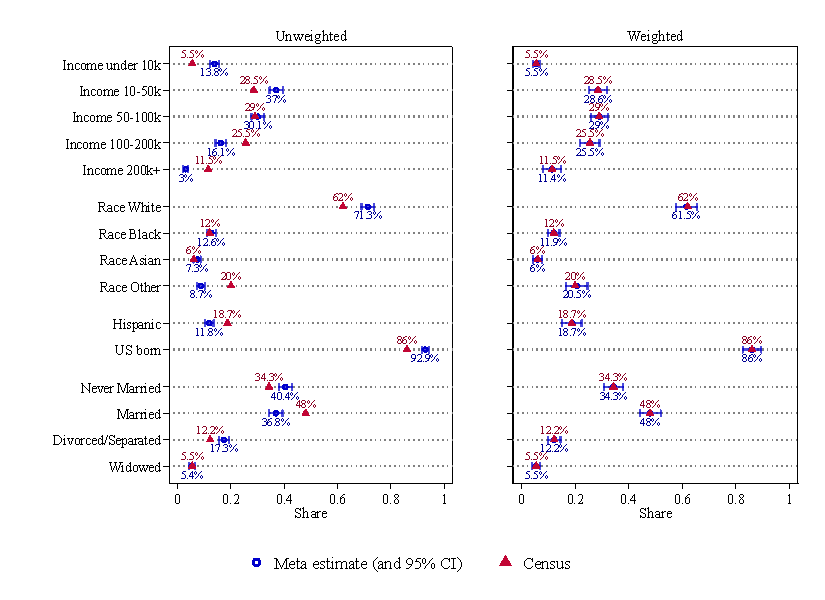
\includegraphics[width=1.1\textwidth]{presentation/Figures/demographics.pdf}
\end{figure}

\subsection{Analysis and Results}
\subsubsection{Method}
There are several ways to quantify the accuracy of survey estimates relative to population benchmarks. Common approaches include squared-error measures such as the root mean squared error (RMSE), chi-squared statistics, and distributional distance measures (e.g., Kullback–Leibler divergence). In this study, we focus on the mean absolute deviation (MAD), also referred to in the related literature as the mean absolute error (MAE) or the average absolute difference, which summarizes the average discrepancy across variables of interest. Formally, let \(\bar{z}_c\) represent the mean value for each variable category \(c\) (e.g., the share of respondents who worked in the previous week) and \(z_c\) denote its benchmark (e.g., Census data or another survey). For a total of \(C\) categories, MAD is defined as:
\begin{equation}
\label{eq_mad}
    \text{MAD} := \frac{1}{C}\sum_c \lvert \bar{z}_c - z_c \rvert.
\end{equation}
MAD is widely used because it is easily interpretable, less sensitive to outliers than squared-error metrics, and directly expresses average deviations in percentage points. It has been recommended in the forecasting literature as a robust accuracy measure \citep{hyndman2006another}, employed in survey methodology to evaluate weighting and calibration \citep{kalton2003weighting, lee2009estimation, brick2011future}, and adopted in practice by survey organizations such as the Pew Research Center \citep{mercer2017weighting}. This makes MAD a natural and transparent choice for evaluating the representativeness of our ad-recruited sample.

For the analysis, we transform survey responses into a common set of binary and continuous variables. For each categorical item, we construct binary indicators coded as 1 if the respondent selected a given category and 0 otherwise, excluding ``Don’t know'' and missing responses. This approach yields a consistent representation of categorical outcomes across benchmarks and the Meta sample. The only exception is the question on time spent on the internet (measured in minutes per day), which we retain as a continuous variable but normalize to the unit interval using a min–max transformation. This standardization ensures comparability across surveys and prevents differences in raw scales from mechanically affecting the computation of discrepancies.







\subsubsection{Strata and Demographic Variables}
Applying \eqref{eq_mad} to the unweighted means of the stratification variables reported in Figure~\ref{fig:strata}, we obtain a MAD of 3.5 percentage points (p.p.). Extending the calculation to the additional sociodemographic variables in Figure~\ref{fig:demographics}—which were not included in the stratification during recruitment—raises the MAD to 6.3 p.p. This gap reflects that the stratification procedure accounted only for the former set of covariates.
After reweighting the Meta sample using the full set of stratification and sociodemographic characteristics (post-stratification weighing), the resulting MAD values are virtually zero, indicating that the \textit{raking} procedure has been correctly applied. 

The magnitude of the MAD naturally evolves over time as additional respondents join the study. This dynamic illustrates the fundamental trade-off between precision and cost that underlies our methodology. Figure~\ref{fig:MAD-strata-demo} plots the unweighted MAD values for both stratification and additional sociodemographic variables across increasing sample sizes, alongside the corresponding acquisition costs per participant (ad cost per final respondent).

The figure shows that as more respondents complete the survey, the MAD for stratification variables declines: starting at roughly 7 p.p. for the first 100 participants and stabilizing at 3.5 p.p. once the sample reaches around 900 respondents. Beyond this point, the MAD remains essentially flat. In contrast, acquisition costs exhibit the opposite trend, beginning at about \$3 per survey participant and rising to approximately \$9 by the end of the study. The trade-off is therefore clear: beyond roughly 900 respondents, further reductions in MAD—i.e., greater precision in representing the stratification variables—do not justify the sharply increasing recruitment costs. Consequently, the optimization engine ceases allocating additional budget to the most expensive strata.\footnote{We observe substantial heterogeneity in acquisition costs across strata, ranging from about \$0.70 for urban, young, mid-educated men to roughly \$20 for urban, middle-aged, low-educated men.} Such cost-sensitive adjustments would not be feasible without detailed real-time information on recruitment expenses.

\begin{figure}[t]
\caption{MAD for Strata, Socio-demographics, and Acquisition Costs Over Time}
        \label{fig:MAD-strata-demo}
        \centering
        \vspace*{0.2cm}
\includegraphics[width=1\textwidth]{presentation/Figures/mad_linear_acquisition_costs_strata and demo.png}
\end{figure}


The orange line in Figure~\ref{fig:MAD-strata-demo} reports results for a set of additional sociodemographic variables not directly included in the stratification. By the end of the recruitment process, the unweighted MAD for these variables is 6.3 p.p. Although higher than the MAD for the stratification variables—reflecting their exclusion from the optimization process—the figure still shows a gradual improvement in precision over time. %Figure~\ref{fig:demographics} provides category-level detail, indicating that lower-income, White, and U.S.-born individuals are somewhat overrepresented relative to Census benchmarks. For the outcome analysis, we apply \textit{raking} to weight the sample to both stratification and sociodemographic benchmarks.\footnote{As expected, the MAD for \textit{weighted} stratification and sociodemographic variables is virtually zero.}



\subsubsection{Outcome Variables}
As discussed above, the outcome survey covered seven domains: socioeconomic status, life satisfaction and perceptions, privacy concerns, attitudes on social issues, internet use, trust, and past voting behavior. We evaluate the accuracy of our methodology both in aggregate across all outcomes and separately within each domain.


\begin{table}[h]
\centering
\caption{Mean Absolute Deviations (MAD) by Domain}
\label{tab:mad_outcomes}
\vspace{0.5cm}
\begin{tabular}{l cc}
\hline\hline
\textbf{Domain} & \multicolumn{2}{c}{\textbf{MAD}} \\
\cline{2-3}
       & \textit{Unweighted} & \textit{Weighted} \\
\hline \vspace{-0.3cm} \\
\vspace{0.5cm}Overall (all outcomes)        & 0.0625 & 0.0608 \vspace{-0.3cm} \\ \hdashline
Past Voting Behavior          & 0.0336 & 0.0326 \\
Privacy Concerns              & 0.0457 & 0.0413 \\
Life Satisfaction/Perceptions & 0.0541 & 0.0493 \\
Socioeconomic Status          & 0.0482 & 0.0500 \\
Attitudes on Social Issues    & 0.0692 & 0.0699 \\
Internet Use                  & 0.0893 & 0.0876 \\
Trust                         & 0.1063 & 0.1053 \\
\hline\hline
\end{tabular}
\end{table}

Table~\ref{tab:mad_outcomes} summarizes the accuracy of our methodology across all outcomes as well as within each domain. The overall MAD is around 6.1-6.2 p.p., with little difference between unweighted and weighted estimates, indicating that reweighting does not substantially alter the alignment of our sample with benchmark surveys. This overall level of accuracy is consistent with prior research comparing convenience-based web samples to probability benchmarks (\citealt{goel2015non, yeager2011comparing, Mercer2018}). Variation across domains, however, is more pronounced. Past voting behavior and privacy concerns display the lowest deviations (around 3–4 p.p.), suggesting that our recruitment strategy captured these outcomes relatively well. Life satisfaction, perceptions, and socioeconomic indicators show slightly higher deviations (around 5 p.p.), while attitudes on social issues and internet use deviate further (7–9 p.p.). The largest discrepancies are observed in trust-related items, with MADs exceeding 10 p.p., underscoring the difficulty of capturing institutional trust in nonprobability samples recruited through social media.



Figure~\ref{fig:MAD-categories} shows the mean absolute deviation (MAD) for overall outcomes and for each domain as the sample size increases from 100 to 1,500 participants. Overall representativeness improves markedly, with the MAD falling from 0.103 at 100 participants to 0.061 at 1,500 participants—an absolute improvement of about 4.2 p.p., corresponding to a 41\% reduction. The largest gains occur in the early phases of recruitment, after which improvements level off. This pattern reflects our adaptive allocation procedure progressively improving the balance of stratification variables as the sample grows. Figure~\ref{fig:MAD-outcomes} in the Appendix reports the dynamics in MAD for both weighted and unweighted estimates, showing that applying post-stratification weighting techniques to our Meta sample  yields only small improvements in representativeness, with the two series converging closely as the sample size increases.

Turning to the specific domains reported in Figure~\ref{fig:MAD-categories}, past voting behavior and privacy concerns converge quickly to relatively low deviations (around 3–4 p.p.), while socioeconomic status and life satisfaction/perceptions stabilize at roughly 5 p.p. Internet use and attitudes on social issues remain somewhat higher, in the range of 7–9 p.p. Trust-related items—encompassing confidence in others, businesses, and the press—stand out as the most difficult to approximate, with deviations consistently above 10 p.p.  Taken together, the figure shows that although representativeness generally improves with sample size, certain domains remain especially challenging to capture.

\begin{figure}[t]
\caption{MAD for Outcome Domains Over Time}
        \label{fig:MAD-categories}
        \centering
        \vspace*{0.1cm}
\includegraphics[width=1\textwidth]{presentation/Figures/MAD_categories.pdf}
\end{figure}


Specific item-level results for each domain are reported in Appendix Figures~\ref{fig:ses} to \ref{fig:voting}. Compared to benchmark surveys, Meta respondents spend more time on the internet and social media, report lower trust in others and less confidence in businesses and the press, express more conservative attitudes toward women and immigrants, perceive lower job security and financial satisfaction, and express less concern about privacy.



These patterns underscore that while the methodology achieves strong overall alignment with benchmarks, certain domains remain inherently more difficult to approximate, providing guidance for where future refinements may be most valuable. The relatively high deviations in internet use are unsurprising given that respondents were recruited through social media, where online activity is systematically higher than in the general population. By contrast, the larger discrepancies observed in attitudes on social issues and in measures of trust—such as confidence in the press, confidence in businesses, and generalized trust in others—likely reflect deeper predispositions of social media users. These attitudinal and institutional dimensions are less amenable to correction through demographic stratification alone, underscoring a persistent challenge in extending nonprobability social media samples to more representative population estimates.


%Figure \ref{fig:MAD-outcomes} reports the MAD for both weighted and unweighted estimates. At the end of the recruitment process, the MAD for both approaches is very similar, remaining below 6.5 percentage points (p.p.). This indicates no significant improvement from applying ex-post weighting to our estimates, consistent with the fact that the sample was already optimized for several weighting variables via stratification. In both cases, the MAD decreases as the recruited sample grows and the underlying stratification improves. 

%The MAD value of 6.3 p.p. for the weighted estimates aligns with findings in the literature comparing convenience opt-in samples recruited through the web to probability-based benchmarks (\citealt{Goel2015, yeager2011comparing, Mercer2018}).



%Notably, MAD values exhibit substantial heterogeneity across outcome categories. Figure~\ref{fig:MAD-categories} illustrates this variation, displaying the MAD for seven outcome categories alongside the combined MAD. Our methodology achieves higher performance for socio-economic and political variables and privacy concerns, with MAD values ranging between 2 and 5.5 p.p. However, the precision is lower for outcomes related to attitudes, trust, and internet usage, where the MAD is between 7 and 11 p.p. Specifically, compared to benchmark surveys, Meta respondents spend more time on the internet and social media, report lower trust in others and less confidence in businesses and the press, exhibit more conservative attitudes toward women and immigrants, report lower job security and financial satisfaction, and express less concern about privacy.






\section{Comparison with Prolific and LLM-generated Samples}

To further validate our methodology and contextualize our results, we compare the performance of our Meta sample against two increasingly relevant alternatives: participants recruited through Prolific and large language model (LLM)–generated digital twins. Prolific has become one of the most widely used online platforms for recruiting survey respondents in academic research, particularly in the social sciences and marketing, due to its ease of use and relatively high data quality compared to other convenience panels \citep{palan2018prolific}. At the same time, recent advances in generative AI have introduced the possibility of using LLMs to create digital ``twins'' of human respondents that can simulate survey responses. This novel approach has sparked growing interest in marketing and related fields, with \citet{toubia2025twin} providing one of the first large-scale resources for building and evaluating such twins. 

Specifically, we conducted the same survey administered to Meta participants on Prolific and generated responses from LLM-based digital twins using the Twin-2K-500 dataset \citep{toubia2025twin}. This comparison allows us to interpret the representativeness of our Meta-based methodology not only against a popular human-sourced benchmark, but also against cutting-edge approaches that aim to approximate consumer populations synthetically.
Our Prolific sample consists of 1,197 respondents recruited and surveyed in June–July 2025. Sampling was stratified by age, gender, and race to ensure that the marginal distributions of these variables closely mirror the 2020 U.S. Census. However, apart from these characteristics, no further demographic controls were applied at the recruitment stage. The digital twin dataset contains a similar number of synthetic respondents, generated to match the demographic distribution of the Prolific sample. For both datasets, we apply post-stratification weighting techniques using the same battery of demographic and socioeconomic indicators employed in the Meta sample—namely age, gender, education, settlement type, income, race, ethnicity, and marital status. This harmonized procedure ensures that differences in performance across samples can be attributed to the recruitment source or data-generation method, rather than to inconsistencies in weighting or adjustment strategies. Finally, we apply equation~\eqref{eq_mad} to both unweighted and weighted estimates and compute the MAD relative to benchmark values from the GSS, the CPS, and Pew.

\begin{figure}[h]
\caption{MAD Comparison: Meta, Prolific, and LLM-generated Samples}
        \label{fig:MAD-comparison}
        \centering
        \vspace*{0.1cm}
\includegraphics[width=0.8\textwidth]{presentation/Figures/mad_grouped_meta_prolific_llm.pdf}
\end{figure}

Figure \ref{fig:MAD-comparison} reports the mean absolute deviation (MAD) aggregated across all outcome variables for the three samples—Meta, Prolific, and LLM-based digital twins—under both unweighted and post-stratification weighted specifications. The Meta sample achieves the lowest MAD (0.062 unweighted, 0.061 weighted), followed by Prolific (0.073 unweighted, 0.071 weighted). The digital twins perform substantially worse, with MADs of 0.120 unweighted and 0.111 weighted. Post-stratification weighting reduces discrepancies slightly for all sources, but the relative ranking across samples remains unchanged. In relative terms, Meta’s accuracy is about 15\% better than Prolific and more than 45\% better than the LLM-generated twins. These results indicate that our Meta-based methodology produces estimates that are at least as representative as Prolific participants and markedly closer to benchmarks than LLM-generated twins.



To further analyze where the discrepancies come from, we examine the performance of the surveys across different substantive domains. Figure~\ref{fig:MAD-categories-comparison} breaks down the mean absolute deviation (MAD) by domain, highlighting where differences across samples are most pronounced. The Meta sample consistently yields the lowest or near-lowest MAD across most domains. For past voting behavior, Meta achieves a deviation of 0.033 compared to 0.093 for Prolific and 0.095 for digital twins, showing a clear advantage. A similar pattern holds for privacy concerns (0.041 for Meta vs. 0.057 for Prolific and 0.105 for digital twins) and socioeconomic status (0.050 for Meta vs. 0.059 for Prolific and 0.032 for digital twins, where twins perform particularly well\footnote{This likely reflects the fact that information on respondents’ employment status—an element of the socioeconomic status domain—was directly incorporated into the construction of the digital twin personas.}). In life satisfaction and perceptions, Meta and Prolific are close (0.049 vs. 0.064), while digital twins perform substantially worse (0.156). For attitudes on social issues, Meta and Prolific again perform similarly (0.070 vs. 0.062), while digital twins are higher (0.115). In internet use, Prolific has the lowest deviation (0.067) compared to Meta (0.088) and twins (0.100). Finally, trust-related measures are the most challenging: MADs exceed 0.10 in all samples, with Meta at 0.105, Prolific at 0.107, and digital twins highest at 0.126.


\begin{figure}[H]
\caption{MAD Comparison: Meta, Prolific, and LLM-generated Samples}
        \label{fig:MAD-categories-comparison}
        \centering
        \vspace*{0.1cm}
\includegraphics[width=1\textwidth]{presentation/Figures/mad_grouped_meta_prolific_llm_bydomain.pdf}
\end{figure}


Overall, the figure shows that the Meta sample generally aligns more closely with benchmark surveys than Prolific or digital twins, with particularly strong performance in political behavior and privacy, while internet use is captured slightly better by Prolific. Digital twins underperform substantially in most domains, especially in perceptual and attitudinal measures. Recent work aligns with our findings. \citet{helbing2022digital} emphasize that digital twin models face inherent limitations when representing human behavior, attitudes, and beliefs, as these constructs are often context-dependent and difficult to capture. Similarly, \citet{lin2022human} review the emerging literature on human digital twins and note that behavioral, psychological, and attitudinal dimensions remain especially challenging to approximate due to the variability of human responses. In a complementary vein, \citet{fett2025practical} show that surveys of digital twin applications tend to focus primarily on functional and technical aspects, with relatively little attention to perceptions, trust, or other attitudinal measures. Together, these studies suggest that digital twins systematically underperform in domains requiring nuanced representations of attitudes or perceptions.




\section{Cost Considerations}

Table \ref{costs} reports the costs of our validation exercise in the U.S. study. These numbers demonstrate that our methodology is both affordable and efficient relative to benchmark approaches, although it remains more expensive than widely used platforms such as Prolific.

\begin{table}[h]
\centering
\caption{Comparison of Survey Costs Across Sampling Methods}
\label{costs}
\vspace{0.3cm}
\begin{tabular}{lcc}
\hline\hline
\textbf{Sample Source} &  \textbf{Cost per Question per Respondent} \\
\hline
Meta (ads + incentives)  & \$0.32 \\
GSS (traditional waves) & \$3.00 \\
GSS (Follow-on, 2024 brochure)  & \$6.67 \\
Prolific   & \$0.095 \\
\hline\hline
\end{tabular}
\end{table}

 On average, in the Meta study, advertising costs per participant were \$6.3, ranging from as little as \$0.70 for urban young medium-educated men to as much as \$20 for urban mid-age low-educated men. In addition, participants were incentivized with \$5 Amazon gift cards upon completing the survey. Summing advertising costs and incentives, the cost per final participant was \$11.6, corresponding to a cost per question per respondent of approximately \$0.32. This is substantially lower than the costs reported for the General Social Survey (GSS). Traditional GSS waves have been estimated at around \$3 per respondent per question \citep{goel2015non}, while more recent documentation for the GSS Follow-on web component suggests a cost of about \$20,000 per survey minute, which equates to roughly \$6.67 per question per respondent for a sample of 1,000 cases \citep{norc2024gss}. By comparison, our Prolific study cost approximately \$2.66 per respondent, which corresponds to about \$0.10 per question per respondent. This confirms that the Meta sample was roughly 3 times more expensive than Prolific on a per-question basis, though still far more cost-effective than gold-standard probability surveys.




%Our validation exercise achieved strong results in terms of representativeness and precision for socio-economic and political variables. The methodology’s strengths include its scalability, the ability to dynamically adjust recruitment based on cost and strata targets, and the integration of Census-derived weights into the recruitment process. However, the drawbacks include lower precision for variables outside the stratification, such as attitudes and trust, and higher costs for certain strata, particularly urban mid-age low-educated men. These findings underscore the importance of balancing cost efficiency with representativeness when designing recruitment strategies.

\section{Applications in Other Countries}

Our methodology was applied to conduct 33 studies across 23 countries, leveraging recruitment ads that reached 33,073,461 people and resulted in 166,535 optimized respondents. The results highlight the flexibility and scalability of our approach in achieving diverse recruitment goals. An open dataset with detailed recruitment information has been created to ensure transparency and facilitate further analysis.





Table \ref{country-results} in the Appendix displays the key metrics from the studies, including the number of strata used for recruitment, maximum click-through rates (CTR), the total reach of the ads, the number of respondents who completed the surveys, and the average ad spend per recruited respondent (excluding incentives). For instance, recruitment costs ranged from as little as \$0.24 in India to \$11.07 in Gambia, reflecting substantial variation across countries and demographic groups. Notably, in 80\% of cases, costs were below \$4.
Strata counts varied widely too, from 1 in Serbia to 200 in Romania, with maximum CTRs exceeding 25\% in some cases, such as Macedonia. Overall, the key takeaway from these studies conducted over the past four years is that it is possible to reach and recruit highly stratified samples across multiple countries through digital ad campaigns in a cost-effective manner.


\section{Discussion and Future Work}

This paper introduces and validates a novel methodology for on-demand survey sampling that is demonstrably more accurate than leading digital alternatives and, most critically, globally scalable. Our findings show that by dynamically optimizing ad spend, we can construct highly stratified samples that are not only cost-effective compared to traditional methods but also directly address the geographic and demographic limitations of pre-assembled online panels. The ability to deploy this tool across dozens of countries, from emerging markets to developed economies, represents a significant step forward in survey research.

The primary implication of our work is the democratization of access to high-quality, targeted survey data. This is supported by our U.S. study, where the methodology achieved a mean absolute deviation of about 6.1 p.p. from gold-standard benchmarks, outperforming both a leading online panel (7.1 p.p.) and LLM-based digital twins (11.1 p.p.). This level of accuracy, combined with a cost-effective price point and proven deployment in over 33 studies across 23 countries, presents researchers and practitioners with a novel option that is not constrained by the geographic footprint of existing panels. This methodology unlocks the potential for rapid, multi-country comparative studies, A/B testing of interventions in diverse and ecologically valid contexts, and the study of niche, hard-to-reach populations that are often invisible to standard survey methods. For businesses, this provides a tool for timely consumer insights in fast-growing markets where traditional data collection is often impractical or prohibitively expensive.

However, the methodology has important boundaries. First, by recruiting from a single ecosystem like Meta, we are sampling from a population of social media users, which may introduce biases on outcomes related to digital behavior or trust in institutions. While post-stratification can mitigate this, it cannot eliminate it entirely. Future work could explore recruiting across multiple platforms (e.g., TikTok, YouTube) to mitigate biases specific to any single platform, though it would not resolve the broader limitation of sampling from a population of social media users. Second, our method relies on the ad platform's proprietary algorithms for ad delivery, which introduces a ``black box'' element; we control the budget, but not the precise mechanism of exposure. Finally, as with any tool that involves micro-targeting, researchers must continue to navigate the ethical considerations of data privacy and informed consent.

At the same time, we recognize that there is still significant work to be done. One area for improvement is optimization, particularly in learning the price and more accurately estimating the price function to better predict the cost and time required for recruitment. Time is an important factor—slower recruitment can be more cost-effective—but determining the optimal speed for a given study is not a trivial task. Additionally, we believe that effective advertisements, brand trust-building, and strong incentives can significantly increase response rates.

This work also opens several exciting avenues for methodological innovation. Our current optimization assumes equal variance across strata; a simple extension would be to dynamically measure stratum-specific variance for key outcome variables during recruitment. This would allow the algorithm to allocate more budget to strata that are not just under-sampled, but also exhibit higher variance on the outcomes of interest, moving beyond simple demographic parity to a more sophisticated optimization of estimate precision. An additional extensions would be to dynamically select the stratification variables themselves. By framing stratification as a real-time variable selection problem—where the goal is to identify covariates that most efficiently partition the population to reduce the variance of the population estimator, future algorithms could learn the optimal stratification scheme on the fly. This combination of covariate learning and the ability to micro-target in real time allows for the creation of a user-friendly system that can affordably generate accurate estimates of population parameters, while relaxing the amount of modeling assumptions required from the user. 

%We refer the reader to our companion manuscript and manual \citep{rao2020conducting} for additional case studies, experiments and applications of this methodology.


%The full recruitment dataset provides valuable insights for researchers aiming to replicate or adapt the methodology.

%There are a few things that we believe our results in the last couple of years show quite clearly:

%\begin{enumerate}
%\item It is possible to reach and recruit highly-stratified samples in many countries via digital ad campaigns in a cost-effective manner.
%\item A non-trivial percentage of people reached can be inticed to click on the ad.
%\item Survey recruitment can be optimized in real-time by building software that connects with ad platform and survey platform APIs.
%\end{enumerate}

%Additionally, another important piece of outstanding work is to show that poststratification weighting applied to these surveys delivers results that compare with gold-standard population surveys and that optimizating for post-stratification weighting during recruitment leads to better results than naive recruitment without stratification.


\section*{\normalsize Funding and Competing Interests}
\normalsize The authors have no funding to report. Dante Donati declares no competing interests in this work. Nandan Rao has ownership interests in Virtual Lab LLC, a company that uses the open-source methodology described in this paper to provide paid services.


%\bibliography{bibs/survey-methodology.bib} 


%\bibliography{bibs/survey-methodology}

\printbibliography


\clearpage
\newpage

\appendix


%***************************************
% APPENDIX
%**************************************

\label{appendix:C}
\setcounter{figure}{0}
\renewcommand{\thefigure}{A\arabic{figure}}
\renewcommand{\theHfigure}{A\arabic{figure}} % for 'hyperref'

\renewcommand{\thetable}{A\arabic{table}}
\renewcommand{\theHtable}{A\arabic{table}} % for 'hyperref'


\section*{Appendix}
\section{Survey Platform and Recruitment Material}

\begin{figure}[H]
\caption{Interactive Dashboard}
\centering
 \vspace*{0.1cm}
\label{fig:dashboard}
\includegraphics[width=14cm]{presentation/Figures/vlab-dash-1b.png} \\\vspace{0.5cm}
\includegraphics[width=14cm]{presentation/Figures/vlab-dash-2b.png}
\end{figure}


\begin{figure}[H]
\caption{Ad Banners for the US Study}
 \vspace*{0.1cm}
\label{fig:creatives}
\centering
\includegraphics[width=13cm]{presentation/Figures/US-ad1.png}
\includegraphics[width=13cm]{presentation/Figures/US-ad2.png}
\end{figure}



\setcounter{table}{0}
\renewcommand\thetable{B.\arabic{table}}
\setcounter{figure}{0}
\renewcommand\thefigure{B.\arabic{figure}}

\section{Survey Instrument \label{survey}}



\subsection*{Demographics}

\paragraph{Country of birth (\textit{Source: CPS})}
In what country were you born?
\begin{itemize}[noitemsep,topsep=0pt]
\item United States
\item Outside the US
\end{itemize}

\paragraph{Age in years (\textit{Source: GSS})}
What is your age?
\begin{itemize}[noitemsep,topsep=0pt]
\item Open response: years in numbers
\item Not eligible if under 18
\item Validation: if above 100, prompt to re-enter
\end{itemize}

\paragraph{Sex assigned at birth (\textit{Source: GSS})}
What sex were you assigned at birth?
\begin{itemize}[noitemsep,topsep=0pt]
\item Male
\item Female
\item Don’t know
\item Prefer not to say
\end{itemize}

\paragraph{Current gender identity (\textit{Source: GSS})}
Do you describe yourself as male, female, or transgender?
\begin{itemize}[noitemsep,topsep=0pt]
\item Male
\item Female
\item Transgender
\item None of these
\item Don’t know
\item Prefer not to say
\end{itemize}

\paragraph{Hispanic origin (\textit{Source: GSS})}
Are you of Hispanic, Latino, or Spanish origin?
\begin{itemize}[noitemsep,topsep=0pt]
\item Yes
\item No
\end{itemize}

\paragraph{Race (\textit{Source: CPS})}
What is your race?
\begin{itemize}[noitemsep,topsep=0pt]
\item White
\item Black or African American
\item American Indian or Alaska Native
\item Asian
\item Native Hawaiian or Other Pacific Islander
\item Multiple races
\item Other
\end{itemize}

\paragraph{Highest education level (\textit{Source: CPS})}
What is the highest level of school you have completed or the highest degree you have received?
\begin{itemize}[noitemsep,topsep=0pt]
\item 12th grade, no diploma
\item High school diploma or equivalent
\item Some college but no degree
\item Bachelor’s degree
\item Master’s degree
\item Doctorate degree
\end{itemize}

\paragraph{Marital status (\textit{Source: GSS})}
What is your current marital status?
\begin{itemize}[noitemsep,topsep=0pt]
\item Married
\item Widowed
\item Divorced
\item Separated
\item Never married
\end{itemize}

\paragraph{Household income (\textit{Source: Census})}
In which of these groups did your household income, from all sources, fall last year (2023), before taxes?
\begin{itemize}[noitemsep,topsep=0pt]
\item Under \$10,000
\item \$10,000 to \$50,000
\item \$50,000 to \$100,000
\item \$100,000 to \$200,000
\item \$200,000 or more
\end{itemize}


\subsection*{Socioeconomic Status (SES)}

\paragraph{Household business (\textit{Source: CPS})}
Do you or anyone in your household have a business or a farm?
\begin{itemize}[noitemsep,topsep=0pt]
\item Yes
\item No
\item Don’t know
\end{itemize}

\paragraph{Current enrollment status (\textit{Source: CPS})}
Last week, were you enrolled in a high school, college, or university (either full-time or part-time)?
\begin{itemize}[noitemsep,topsep=0pt]
\item Yes
\item No
\end{itemize}

\paragraph{Any work last week (\textit{Source: CPS})}
Last week, did you do any work for either pay or profit?
\begin{itemize}[noitemsep,topsep=0pt]
\item Yes
\item No
\item Retired
\item Disabled
\item Unable to work
\end{itemize}


\subsection*{Attitudes on Social Issues}

\paragraph{Family life and women’s full-time work (\textit{Source: GSS})}
“All in all, family life suffers when the woman has a full-time job.”
\begin{itemize}[noitemsep,topsep=0pt]
\item Strongly agree
\item Agree
\item Neither agree nor disagree
\item Disagree
\item Strongly disagree
\item Don’t know
\end{itemize}

\paragraph{Affirmative action preferences (\textit{Source: GSS})}
Preferential hiring and promotion of Black people because of past discrimination.
\begin{itemize}[noitemsep,topsep=0pt]
\item Strongly favor
\item Favor
\item Oppose
\item Strongly oppose
\item Don’t know
\end{itemize}

\paragraph{Immigrants and job competition (\textit{Source: GSS})}
“Immigrants take jobs away from people who were born in America.”
\begin{itemize}[noitemsep,topsep=0pt]
\item Strongly agree
\item Agree
\item Neither agree nor disagree
\item Disagree
\item Strongly disagree
\item Don’t know
\end{itemize}


\subsection*{Internet Use}

\paragraph{Web hours per week (\textit{Source: GSS})}
Not counting e-mail, about how many hours per week do you use the Web (including browsing, social media, streaming, chat, online conferencing)?
\begin{itemize}[noitemsep,topsep=0pt]
\item Open response: number of hours
\end{itemize}

\paragraph{Health information online frequency (\textit{Source: GSS})}
During the past 12 months, how often did you use the internet to look for health or medical information for yourself or someone else?
\begin{itemize}[noitemsep,topsep=0pt]
\item Several times a day
\item Once a day
\item Several times a week
\item Several times a month
\item Several times a year
\item Never or almost never
\item Don’t know
\end{itemize}


\subsection*{Privacy Concerns}

\paragraph{Concern about company data use (\textit{Source: Pew})}
How concerned are you about how companies use the data they collect online about you?
\begin{itemize}[noitemsep,topsep=0pt]
\item Very concerned
\item Somewhat concerned
\item Not too concerned
\item Not at all concerned
\item Don’t know
\end{itemize}

\paragraph{Support for potential TikTok ban (\textit{Source: Pew})}
There are worries that the Chinese government could access personal information from American users of TikTok, a social media platform owned by the Chinese company ByteDance. To address these concerns, the U.S. government has recently passed a new law. It requires ByteDance to sell its part of TikTok within a year or else the platform might be banned in the U.S.\\
Do you agree or disagree with the decision to potentially ban TikTok in the U.S. if its Chinese owner does not sell its stake within the next year?
\begin{itemize}[noitemsep,topsep=0pt]
\item Strongly agree
\item Agree
\item Neither agree nor disagree
\item Disagree
\item Strongly disagree
\item Don’t know
\end{itemize}


\subsection*{Trust}

\paragraph{Interpersonal trust (\textit{Source: GSS})}
Generally speaking, would you say that most people can be trusted, or that you can’t be too careful?
\begin{itemize}[noitemsep,topsep=0pt]
\item Can trust
\item Can’t be too careful
\item Depends
\item Don’t know
\end{itemize}

\paragraph{Confidence in major companies (\textit{Source: GSS})}
As far as the people running major companies in this country are concerned, how much confidence do you have in them?
\begin{itemize}[noitemsep,topsep=0pt]
\item A great deal
\item Only some
\item Hardly any
\item Don’t know
\end{itemize}

\paragraph{Confidence in the press (\textit{Source: GSS})}
As far as the people running the press in this country are concerned, how much confidence do you have in them?
\begin{itemize}[noitemsep,topsep=0pt]
\item A great deal
\item Only some
\item Hardly any
\item Don’t know
\end{itemize}

\subsection*{Life Satisfaction/Perceptions}

\paragraph{Self-rated health (\textit{Source: GSS})}
Would you say your own health, in general, is:
\begin{itemize}[noitemsep,topsep=0pt]
\item Excellent
\item Good
\item Fair
\item Poor
\item Don’t know
\end{itemize}

\paragraph{Poorer service frequency (\textit{Source: GSS})}
In your day-to-day life, how often do you receive poorer service than other people at restaurants or stores?
\begin{itemize}[noitemsep,topsep=0pt]
\item Almost every day
\item At least once a week
\item A few times a month
\item A few times a year
\item Less than once a year
\item Never
\item Don’t know
\end{itemize}

\paragraph{Financial satisfaction (\textit{Source: GSS})}
How satisfied are you with your present financial situation?
\begin{itemize}[noitemsep,topsep=0pt]
\item Pretty well satisfied
\item More or less satisfied
\item Not satisfied at all
\item Don’t know
\end{itemize}

\paragraph{Layoff likelihood next 12 months (\textit{Source: GSS})}
Thinking about the next 12 months, how likely is it that you will lose your job or be laid off?
\begin{itemize}[noitemsep,topsep=0pt]
\item Very likely
\item Fairly likely
\item Not too likely
\item Not at all likely
\item Don’t know
\end{itemize}


\subsection*{Past Voting Behavior}

\paragraph{Voted in 2020 (\textit{Source: GSS})}
Do you remember for sure whether or not you voted in the 2020 presidential election?
\begin{itemize}[noitemsep,topsep=0pt]
\item Voted
\item Did not vote
\item Ineligible
\item Don’t know / Can’t remember
\end{itemize}

\paragraph{2020 vote choice (\textit{Source: GSS})}
In the 2020 presidential election, did you vote for:
\begin{itemize}[noitemsep,topsep=0pt]
\item Joe Biden
\item Donald Trump
\item Other candidate
\item Didn’t vote for president
\item Don’t know / Can’t remember
\end{itemize}

\paragraph{Hypothetical 2020 choice (\textit{Source: GSS})}
If you had voted in 2020, who would you have voted for?
\begin{itemize}[noitemsep,topsep=0pt]
\item Joe Biden
\item Donald Trump
\item Other
\item Don’t know / Can’t remember
\end{itemize}







\section{Additional Results}

\label{appendix:C}
\setcounter{figure}{0}
\renewcommand{\thefigure}{C\arabic{figure}}
\renewcommand{\theHfigure}{C\arabic{figure}} % for 'hyperref'

\renewcommand{\thetable}{C\arabic{table}}
\renewcommand{\theHtable}{C\arabic{table}} % for 'hyperref'

\begin{figure}[H]
\caption{Overall MAD for Outcome Variables Over Time}
        \label{fig:MAD-outcomes}
        \centering
        \vspace*{0.1cm}
\includegraphics[width=1\textwidth]{presentation/Figures/MAD_weighted_unweighted.pdf}
\end{figure}

\begin{figure}[H]
\caption{Socio-economic Status}
        \label{fig:ses}
        \centering
        %\vspace*{-0.1cm}
\includegraphics[width=.85\textwidth]{presentation/Figures/cps.pdf}
\end{figure}

\begin{figure}[H]
\caption{Financial Satisfaction and Job Security}
        \label{fig:satisfaction}
        \centering
        %\vspace*{-0.1cm}
\includegraphics[width=.85\textwidth]{presentation/Figures/gss_satisfaction_2024.pdf}
\end{figure}

\begin{figure}[H]
\caption{Perceptions on Health and Services}
        \label{fig:health}
        \centering
        %\vspace*{-0.1cm}
\includegraphics[width=.85\textwidth]{presentation/Figures/gss_health_2024.pdf}
\end{figure}

\begin{figure}[H]
\caption{Attitudes Towards Social Issues}
        \label{fig:social-issues}
        \centering
        %\vspace*{-0.1cm}
\includegraphics[width=.85\textwidth]{presentation/Figures/gss_attitudes_2024.pdf}
\end{figure}


\begin{figure}[H]
\caption{Trust in Others, Businesses and the Press}
        \label{fig:trust}
        \centering
        %\vspace*{-0.1cm}
\includegraphics[width=.85\textwidth]{presentation/Figures/gss_trust_2024.pdf}
\end{figure}



\begin{figure}[H]
\caption{Internet Use}
        \label{fig:internet}
        \centering
        %\vspace*{-0.1cm}
\includegraphics[width=.85\textwidth]{presentation/Figures/gss_internet.pdf}
\end{figure}

\begin{figure}[H]
\caption{Internet Use for Health Information}
        \label{fig:internet}
        \centering
        %\vspace*{-0.1cm}
\includegraphics[width=.85\textwidth]{presentation/Figures/gss_internet_medical.pdf}
\end{figure}


\begin{figure}[H]
\caption{Privacy Concerns}
        \label{fig:social-issues}
        \centering
        %\vspace*{-0.1cm}
\includegraphics[width=.85\textwidth]{presentation/Figures/gss_privacy.pdf}
\end{figure}


\begin{figure}[H]
\caption{Past Voting Behavior}
        \label{fig:voting}
        \centering
        %\vspace*{-0.1cm}
\includegraphics[width=.85\textwidth]{presentation/Figures/gss_voting_2024.pdf}
\end{figure}

\begin{table}[t]
    \centering
    \caption{Results from 24 Countries}
        \label{country-results}
    \vspace*{0.2cm}
\begin{tabular}{llrlrrl}
\toprule
 & Country & Strata & Max CTR & Reach & Respondents & Average Ad Cost \\
\midrule
0 & India & 24 & 5.09\% & 873653 & 9130 & \$0.24 \\
1 & Libya & 176 & 27.1\% & 1000294 & 8338 & \$0.3 \\
2 & Lebanon & 48 & 15.03\% & 1370234 & 17399 & \$0.57 \\
3 & Jordan & 192 & 10.05\% & 2223793 & 17223 & \$0.6 \\
4 & Iraq & 144 & 8.58\% & 4280255 & 16015 & \$0.61 \\
5 & Serbia & 48 & 13.58\% & 985109 & 13995 & \$0.67 \\
6 & Nigeria & 23 & 6.42\% & 145437 & 2393 & \$0.75 \\
7 & US & 10 & 13.61\% & 16849 & 1118 & \$0.85 \\
8 & US & 4 & 6.9\% & 10616 & 316 & \$0.87 \\
9 & Haiti & 16 & 10.0\% & 1218842 & 10491 & \$0.94 \\
10 & Honduras & 144 & 7.4\% & 909597 & 4922 & \$0.95 \\
11 & Lebanon & 48 & 13.82\% & 1650052 & 14354 & \$1.03 \\
12 & Papa New Guinea & 64 & 8.71\% & 118980 & 1825 & \$1.46 \\
13 & Iraq & 80 & 8.27\% & 5616663 & 6520 & \$1.55 \\
14 & US & 14 & 6.14\% & 120647 & 2553 & \$1.66 \\
15 & Ukraine & 64 & 5.17\% & 648512 & 2394 & \$1.69 \\
16 & Kyrgyzstan & 24 & 9.63\% & 489054 & 3004 & \$1.76 \\
17 & Djibouti & 16 & 10.84\% & 313493 & 2252 & \$2.19 \\
18 & Kosovo & 56 & 19.93\% & 663059 & 6084 & \$2.46 \\
19 & Chad & 32 & 7.59\% & 327048 & 2305 & \$2.64 \\
20 & Jamaica & 16 & 15.03\% & 482097 & 4105 & \$2.72 \\
21 & Belize & 24 & 9.1\% & 43684 & 264 & \$2.89 \\
22 & Serbia & 1 & 6.75\% & 342403 & 1737 & \$2.99 \\
23 & Macedonia & 32 & 24.58\% & 384956 & 3156 & \$3.19 \\
24 & Romania & 200 & 9.31\% & 785811 & 1863 & \$3.23 \\
25 & Macedonia & 32 & 25.17\% & 538295 & 4565 & \$3.26 \\
26 & Jordan & 96 & 7.14\% & 1304979 & 2146 & \$3.72 \\
27 & US & 16 & 3.93\% & 241134 & 1429 & \$4.55 \\
28 & Nigeria & 120 & 7.75\% & 563939 & 177 & \$5.55 \\
29 & Bulgaria & 8 & 3.91\% & 170205 & 170 & \$6.16 \\
30 & Cameroon & 80 & 11.85\% & 1427793 & 1712 & \$6.72 \\
31 & India & 160 & 5.77\% & 3526970 & 1639 & \$7.85 \\
32 & Gambia & 2 & 5.86\% & 279008 & 697 & \$11.07 \\
\bottomrule
\end{tabular}
\end{table}



\end{document}